% Upload the three PNG files into an updated_figures/ folder beside your main
% .tex file. Replace the existing figure environments; do not append duplicates.
% Requires \usepackage{graphicx}. Keep the existing labels below so references
% continue to resolve. Wide floats preserve label readability in two columns.

\begin{figure*}[!t]
    \centering
    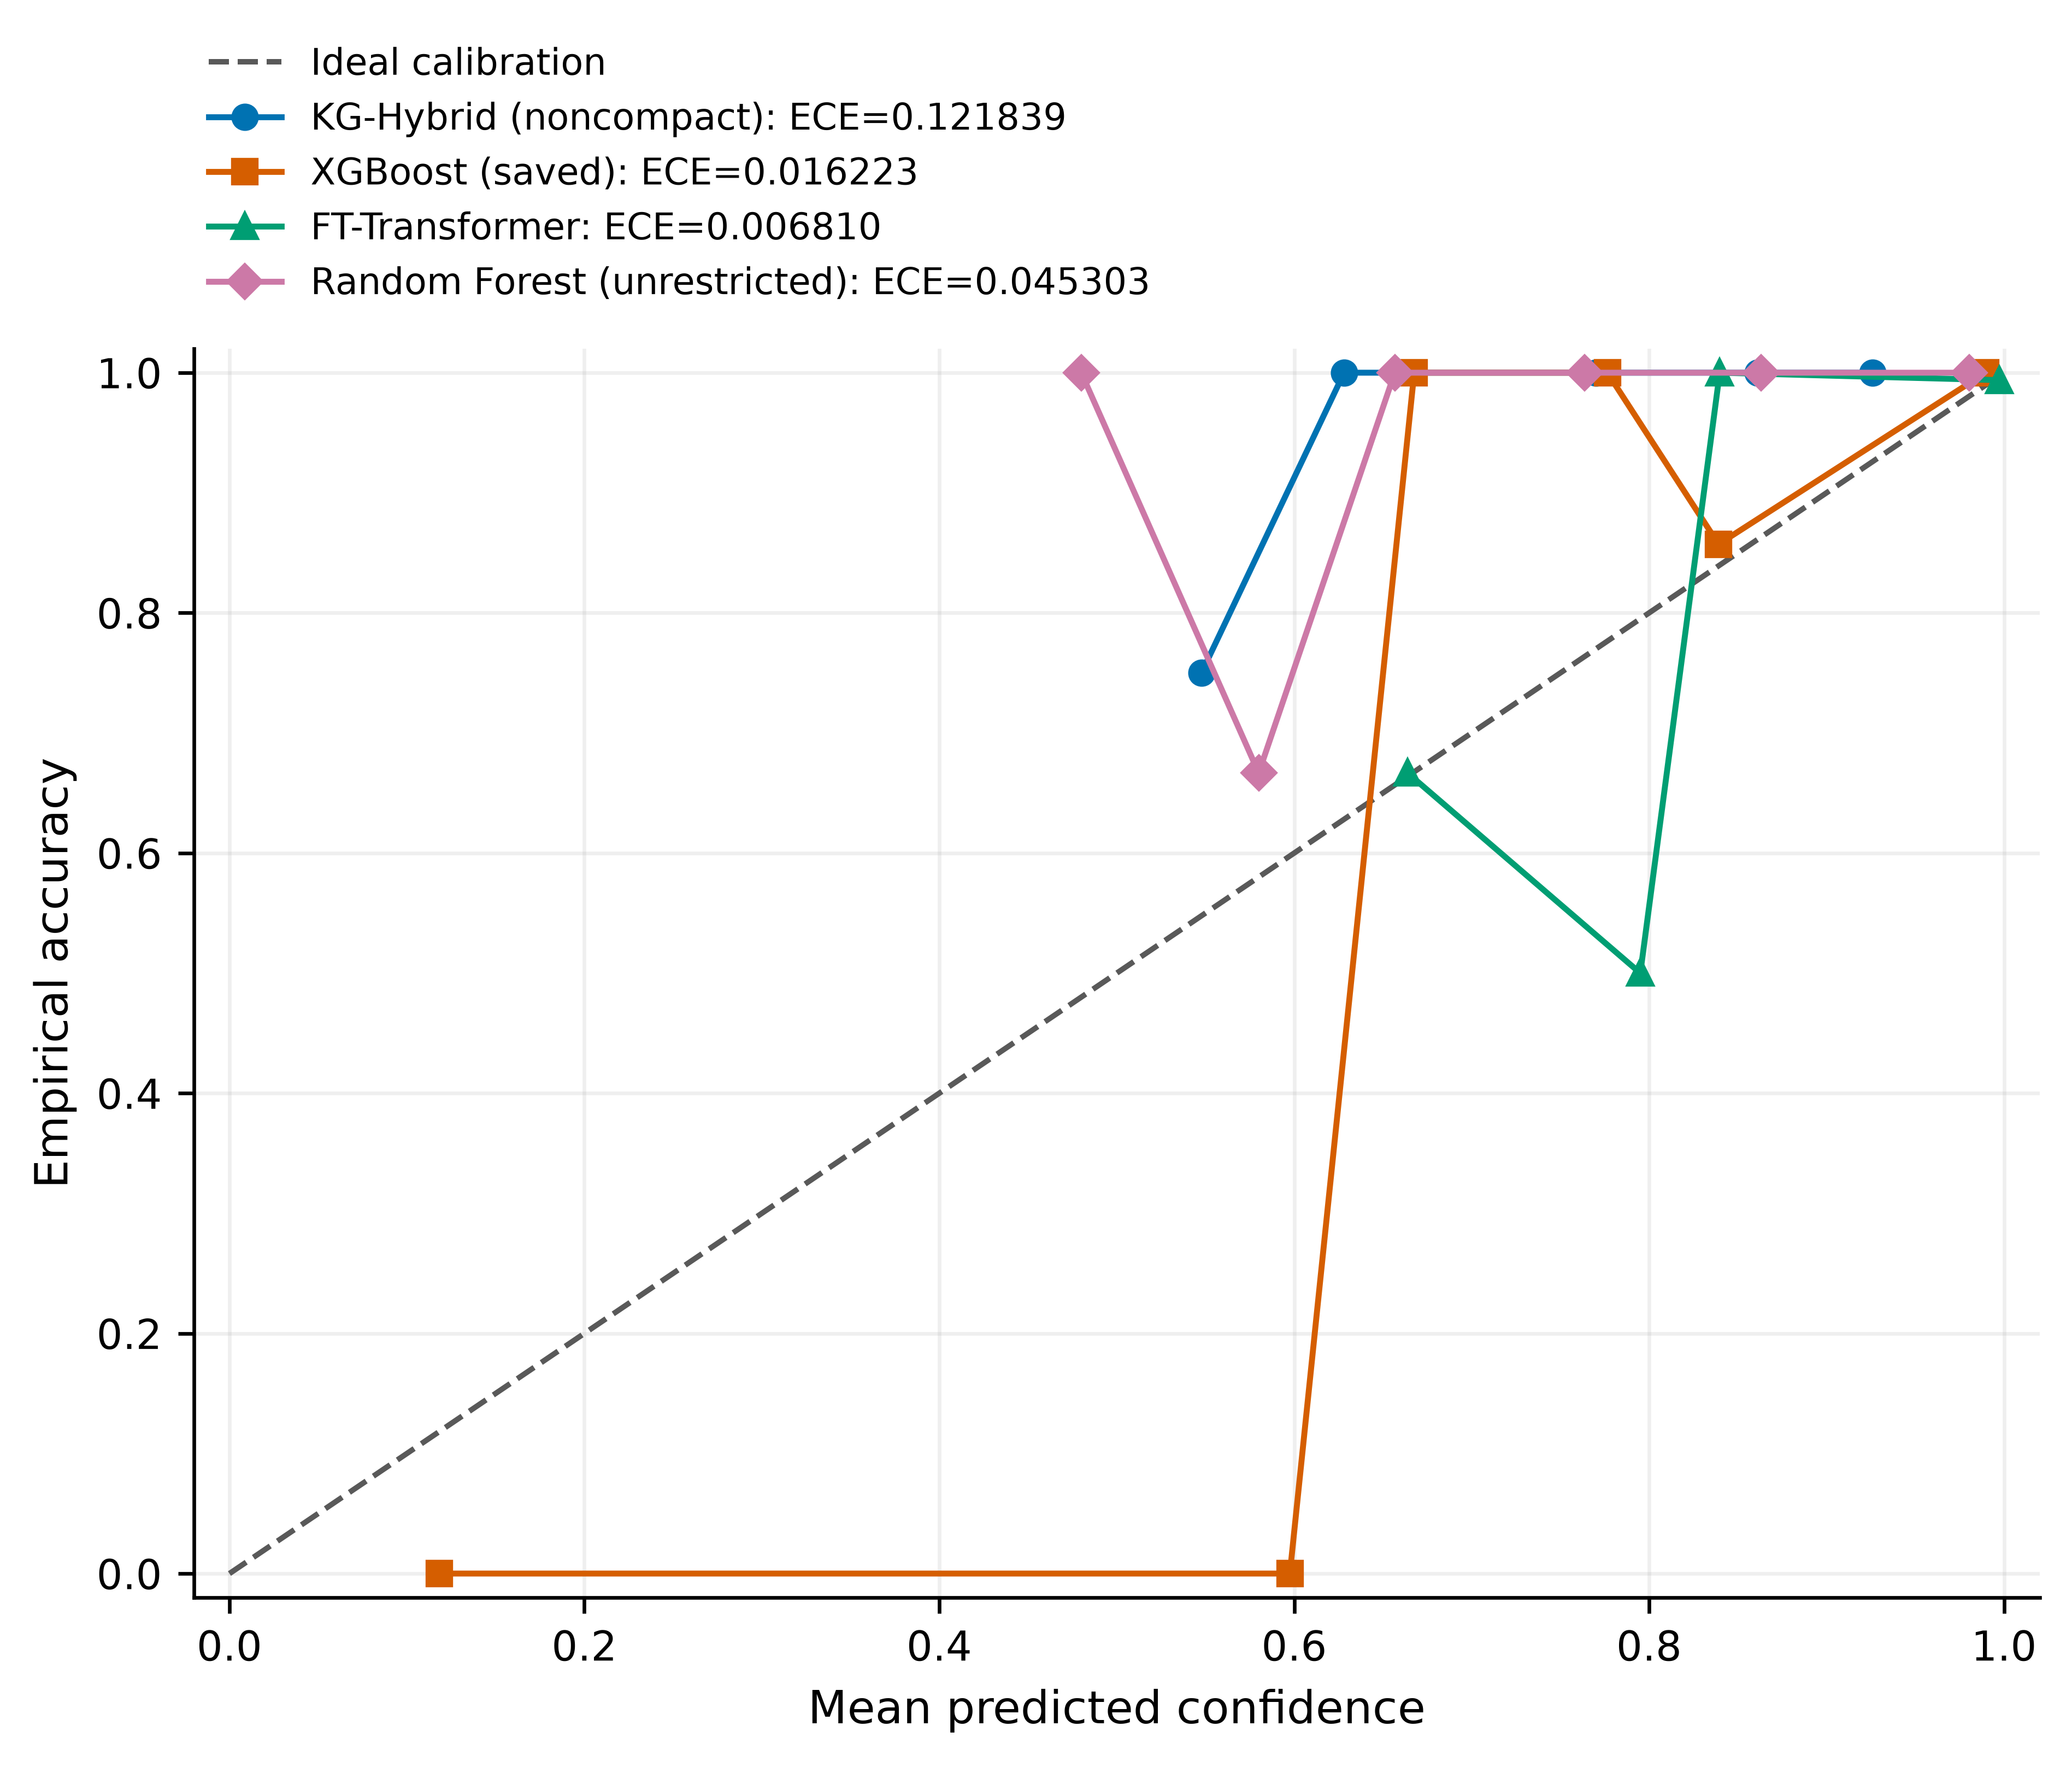
\includegraphics[width=0.80\textwidth]{updated_figures/fig1_reliability_saved_checkpoint.png}
    \caption{Top-label reliability diagram for the designated 330-record
    saved-checkpoint test partition. Markers indicate empirical accuracy and
    mean predicted confidence within populated bins from ten equal-width
    confidence bins; lines connect the populated-bin summaries. The dashed
    diagonal represents ideal calibration. ECE values are computed from the
    same saved probability arrays used in Table~V. The Random Forest curve
    uses the unrestricted configuration. This evaluation is separate from
    the compact five-seed comparison.}
    \label{fig:reliability}
\end{figure*}

\begin{figure*}[!t]
    \centering
    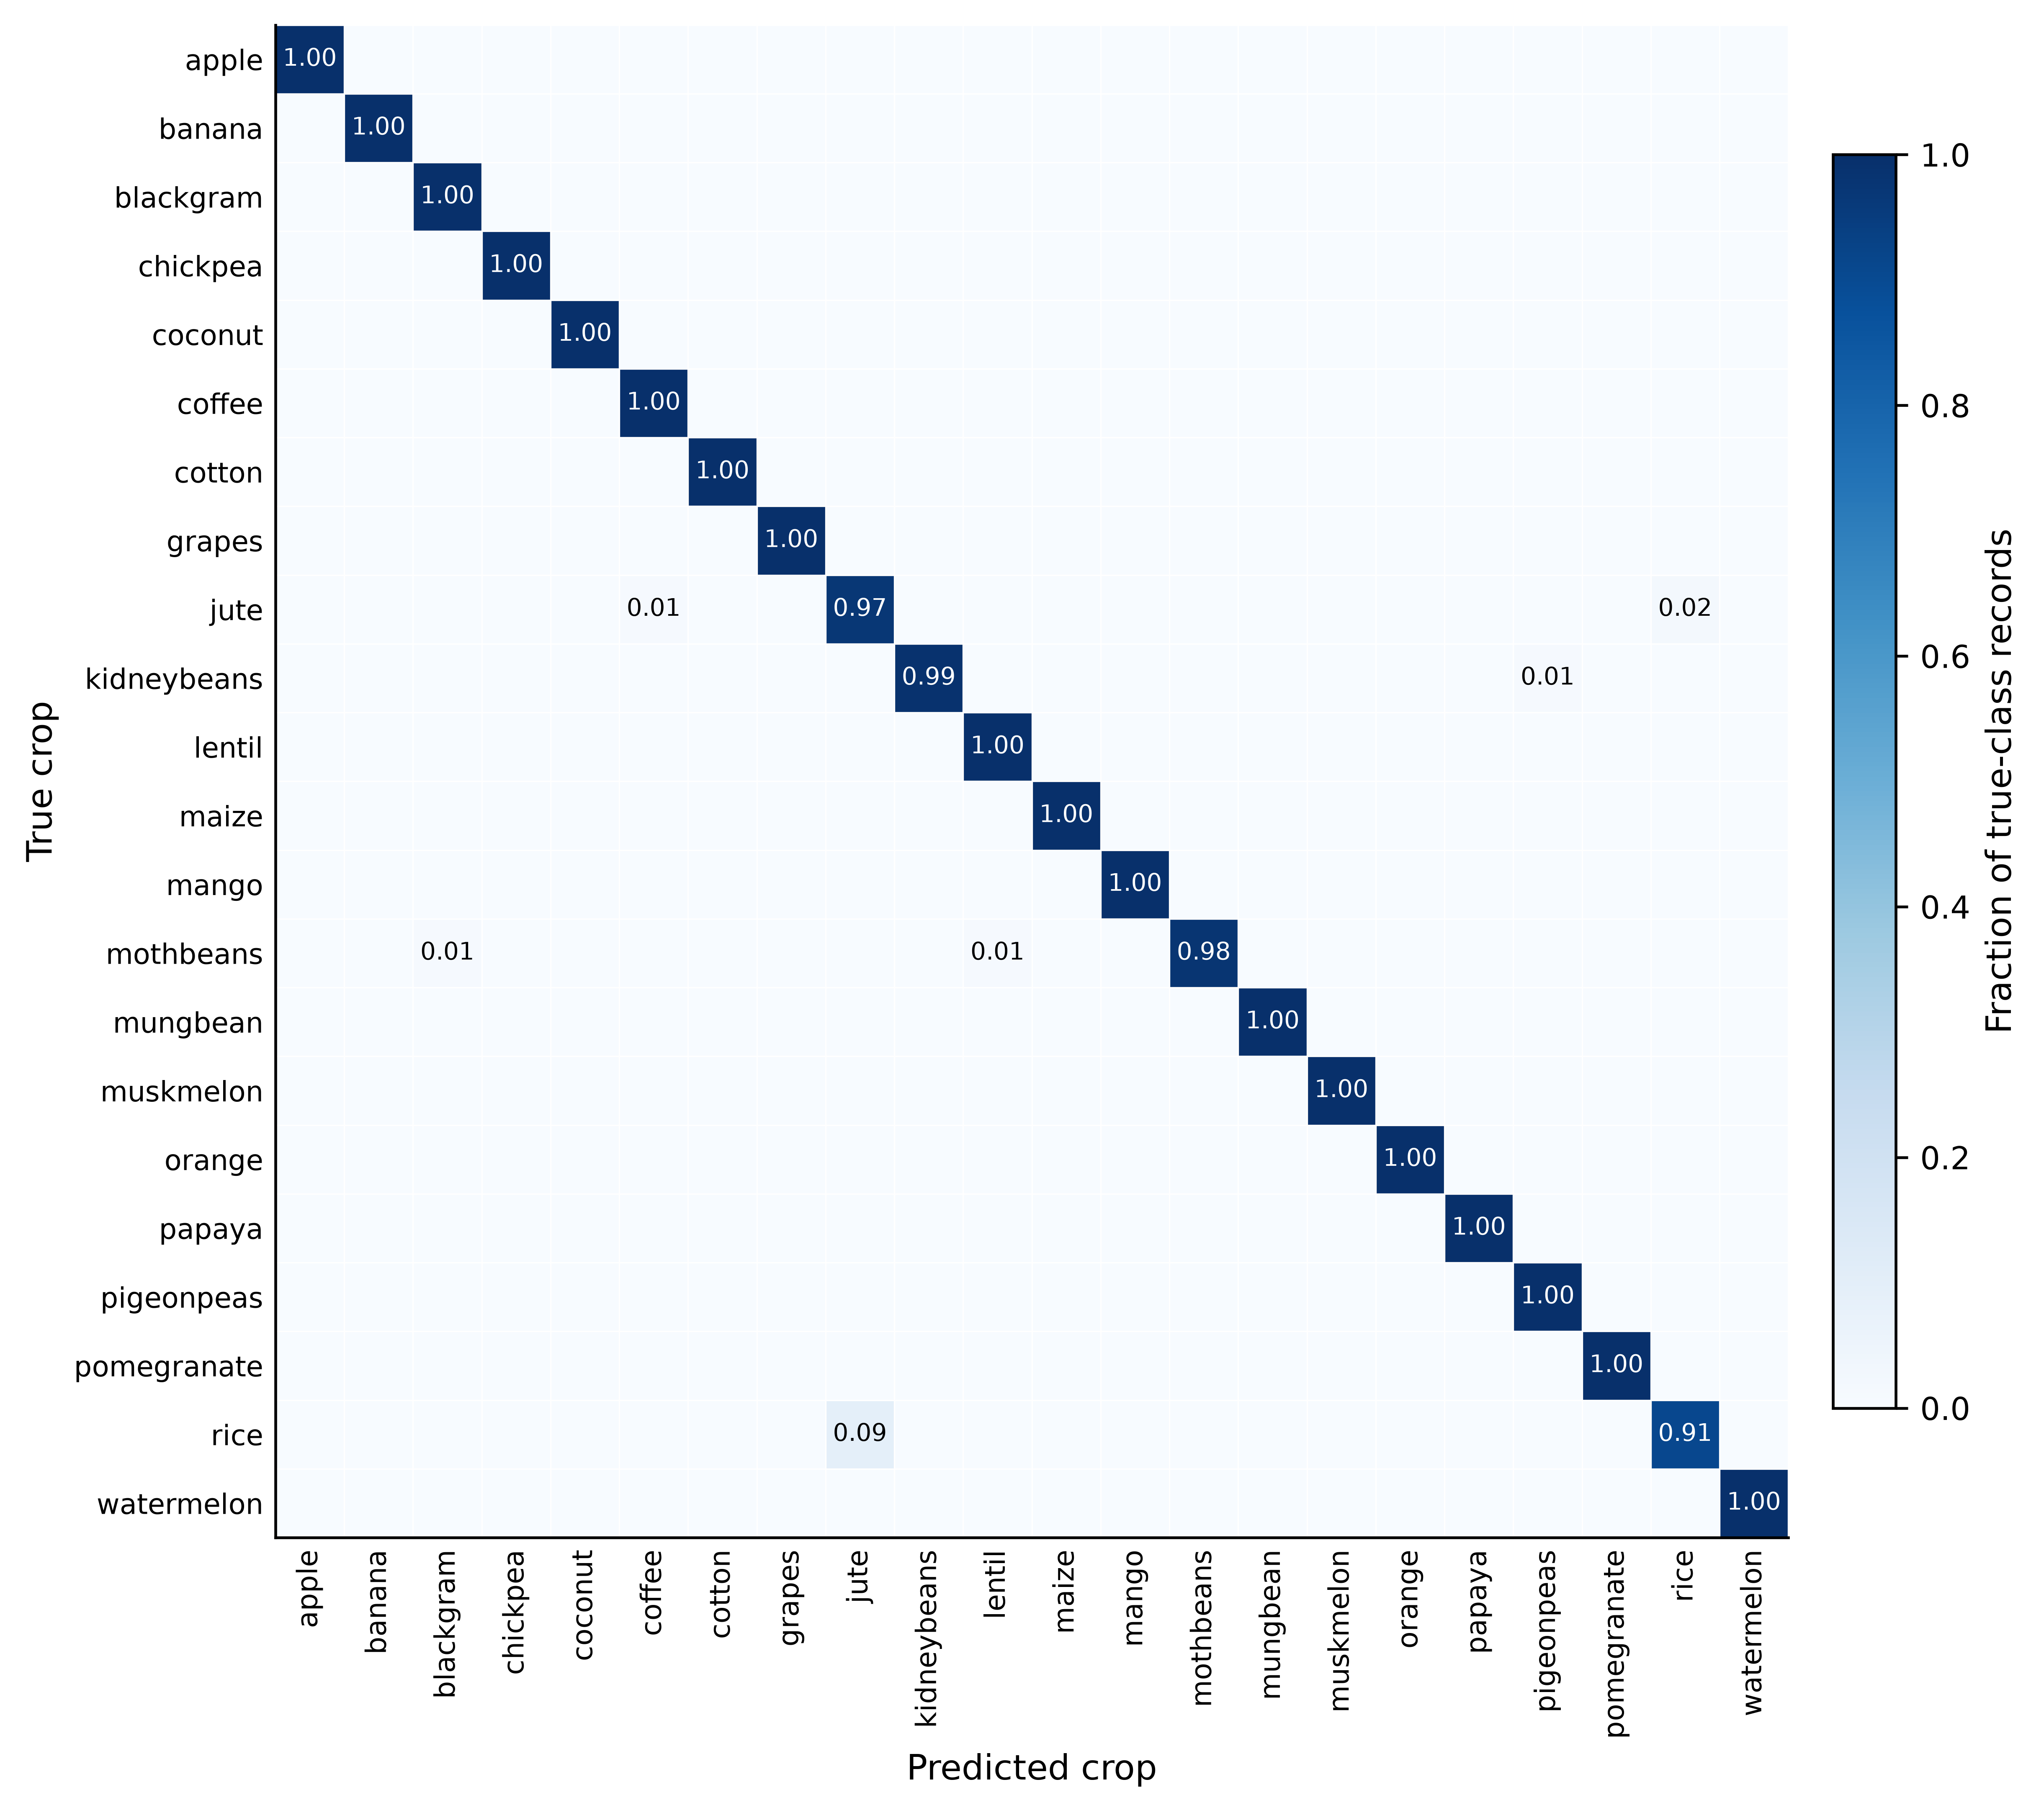
\includegraphics[width=0.98\textwidth]{updated_figures/fig2_confusion_oof_normalized.png}
    \caption{Row-normalized KG-Hybrid confusion matrix pooled across the
    completed noncompact five-fold cross-validation experiment. Each of the
    22 classes contributes 100 out-of-fold records, giving 2,200 predictions
    in total. Rows denote true classes and columns denote predicted classes;
    nonzero entries show fractions of the corresponding true-class records.
    The pooled predictions contain 2,185 correct classifications and 15
    errors. This matrix is not derived from the compact-model test splits.}
    \label{fig:confusion}
\end{figure*}

\begin{figure*}[!t]
    \centering
    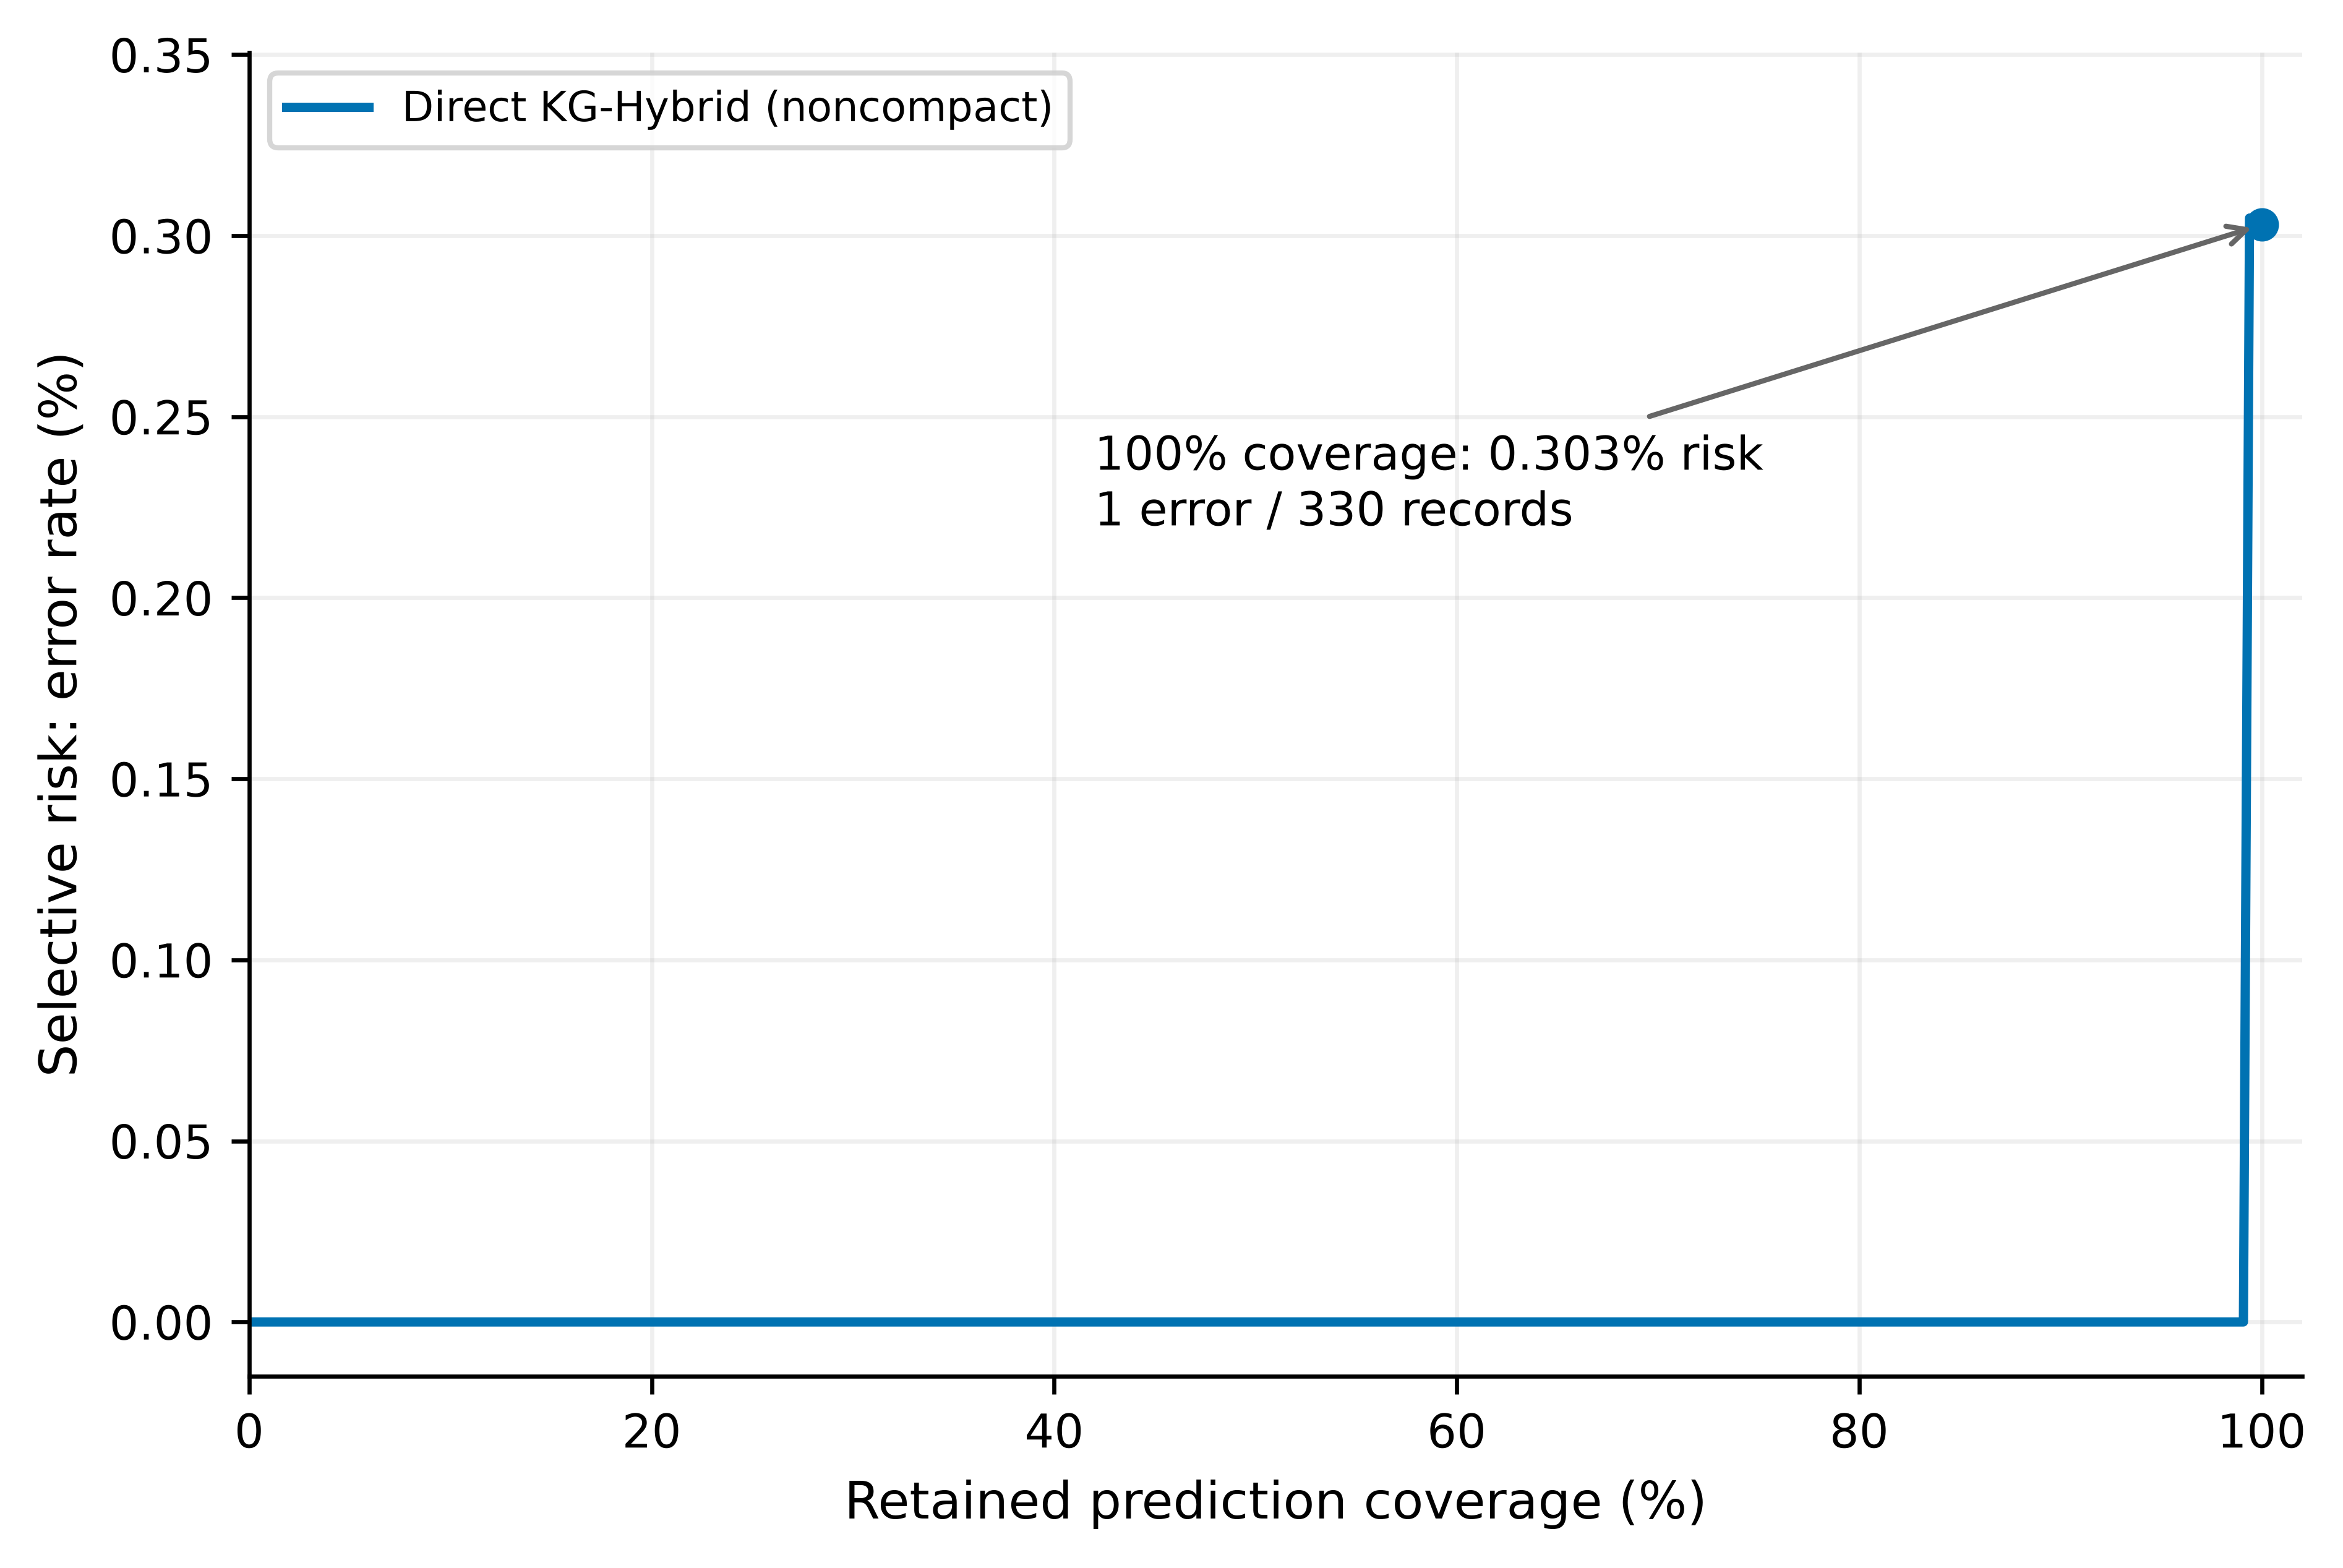
\includegraphics[width=0.80\textwidth]{updated_figures/fig3_risk_coverage_direct_hybrid.png}
    \caption{Selective risk--coverage curve for direct corrected noncompact
    KG-Hybrid predictions on the designated 330-record test partition.
    Predictions are retained when their maximum class probability meets a
    varying confidence threshold, with tied confidence values retained
    together. Coverage is the percentage of retained records, and risk is
    their classification error rate in percent. At full coverage, one error
    among 330 records gives approximately 0.303\% risk. The curve excludes
    XGBoost early-exit routing, MC-Dropout sampling, and latency measurements.}
    \label{fig:risk_coverage}
\end{figure*}
